\chapter{BGP MRAI dependency}
\label{cha:bgp_mrai_experiments}

\ac{MRAI} is one of the parameters that mostly has caused divergences in the
scientific community.
And, after the introduction in the protocol since version 4 \cite{rfc4271}
is one of the parameter more studied for it multiple effects, the correct setting
can improve the protocol performances, while, an incorrect one can generate
exponential convergence behaviours even in small network
\cite{fabrikant2011there,griffin2001experimental}.

The protocol strictly depends on this parameter, because as we saw in \Cref{cha:bgp_fsm},
the incorrect use of it can lead to tremendous consequences, even worst of not
having it at all.
In other cases, with a particular setting of it is possible to improve the network
performances.
Recent studies about centrality metrics on routing protocols introduce, through
the distributed computation of the metric, to a
timer trade-off improvement \cite{MaLo18_ToN,GhiMa18_infocom}.
This kind of approach has been also applied on \ac{BGP} with positive results on
network failures \cite{milani2019BGP,milani2020improving}.

All those study points out how we can set \ac{MRAI} to improve network
performances, but what about how \ac{MRAI} reacts to different problems?
Is it possible that \ac{MRAI} reacts differently based on where the signal
occurs?
In fact, our hypothesis is that is not enough just look to the \ac{MRAI} setting
because other factors can be relevant too.
For example, a change near the central clique of $T$ nodes could provoke a large
storm of messages because \ac{MRAI} doesn't affect in time the spreading of information.
While a change in the periphery could be cushioned without it reaching the center
of the network multiple times.

\section{Clique Experiments}
\label{sec:bgp_mrai_clique}

The clique topology is one of the worst-case scenarios as specified in Labovitz et al.
\cite{labovitz2000delayed}.
For this reason I decided to start my study from it.
I used two approaches in this Environment, the first one keeps the \ac{IW} active
the second one doesn't use of this property.
To emphasize the effects of this parameter with the effects also of different
\ac{MRAI} settings.

The Environment properties are listed in \Cref{tbl:clique_properties}

\begin{table}[h]
	\begin{center}
	\begin{tabular}{ || m{4cm}| m{8cm} || } 
	\hline
	Property & Value \\ 
	\hline \hline
	Seeds & $[1, 10]$ \\ 
	\hline
	Signaling & \q{AW} \\
	\hline
		Withdraws delay & Uniform distribution between \SI{1}{\second} and \SI{5}{\second} \\ 
	\hline
	Announcement delay & constant distribution of \SI{5}{\second} \\ 
	\hline
		MRAI & $[0, 60]$ \\
	\hline
	Link delay & Uniform distribution between \SI{0.0001}{\second} and \SI{0.5}{\second} \\
	\hline
	\end{tabular}
\end{center}

	\caption{Clique environment properties}
    \label{tbl:clique_properties}
\end{table}

As described in \Cref{tbl:clique_properties}, for each \ac{MRAI} value has been
executed \num{10} different runs of the environment.
The clique graph used in these experiments is composed of \num{15} nodes.
The \ac{MRAI} strategy used is the \textit{fixed} one, so every link will have the
same \ac{MRAI} value.
The results are presented in \Cref{fig:clique_evolution}

\begin{figure}[h]
     \centering
     \begin{subfigure}[b]{0.45\textwidth}
         \centering
         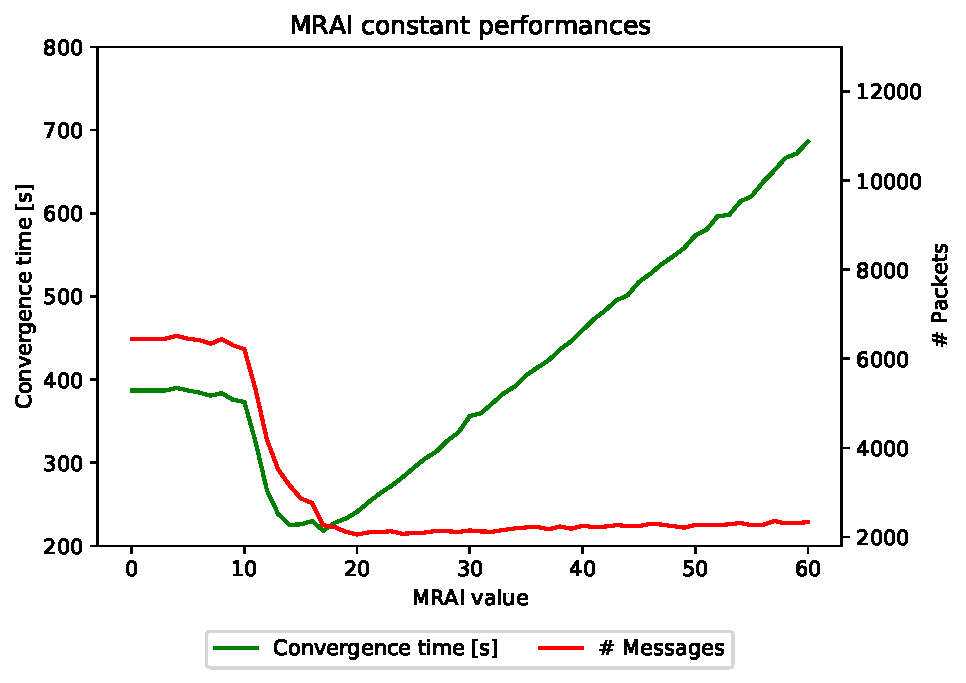
\includegraphics[width=\textwidth]{images/clique/messagesVStime/pareto-clique-constant_mrai_evolution.pdf}
		 \caption{Network performances \textbf{with} \textbf{\ac{IW}}}
         \label{fig:clique_evolution_IW}
     \end{subfigure}
     \hfill
     \begin{subfigure}[b]{0.45\textwidth}
         \centering
         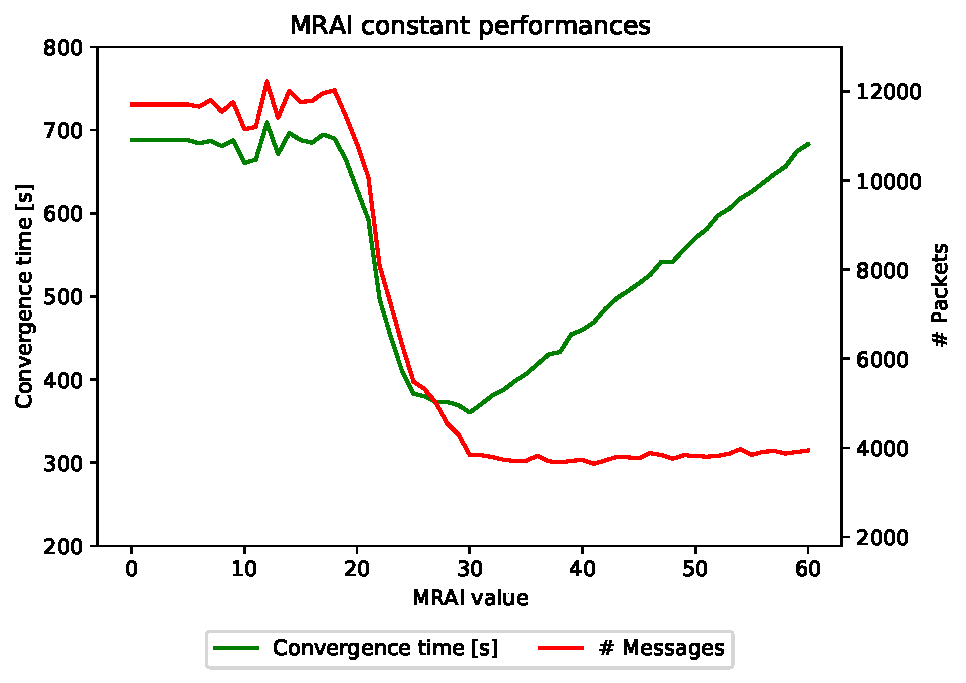
\includegraphics[width=\textwidth]{images/clique/messagesVStime/pareto-clique-noIW-constant_mrai_evolution.pdf}
		 \caption{Network performances \textbf{without} \textbf{\ac{IW}}}
         \label{fig:clique_evolution_noIW}
     \end{subfigure}
		\caption{Evolution of the network performances on the clique graph of \num{15}
			nodes using a fixed \ac{MRAI} from \num{0} to \num{60} seconds.}
        \label{fig:clique_evolution}
\end{figure}

Is possible to notice in \Cref{fig:clique_evolution} both the effect of \ac{MRAI}
and \ac{IW}.
Those plots represent the network performances in terms of convergence time and
number of messages transmitted to reach the convergence after the transmission
of the signal \q{AW}.
The convergence time is represented by the average time from all the nodes in the
network.
Each point in the plots is the average of the \num{10} runs with the \textit{fixed}
\ac{MRAI} value on the $x$ axis.
The left $y$ axis should be used with the convergence time, the green line, while
the second $y$ axis represents the number of messages transmitted, the red line.

The effects of \ac{MRAI} are present in both the plots but in two different
moments.
In \Cref{fig:clique_evolution_IW} \ac{MRAI} affects both the convergence time and
the number of messages around \SI{10}{\second} up to \SI{20}{\second}.
After the threshold of \SI{20}{\second}, the effects of \ac{MRAI} are counterproductive,
the convergence time is negatively affected because the nodes start to wait for more
time without obtaining more useful information.
This can be seen also in the number of messages that reaches a constant value.
Are not necessary other messages to converge and also \ac{MRAI} doesn't give
enough information to the node in order to reduce again the transmitted messages.

In \Cref{fig:clique_evolution_noIW} we can see the same effect but with a higher
\ac{MRAI} value.
The number of transmitted messages reaches the constant value with an \ac{MRAI}
value around \SI{30}{\second}.
The effects of \ac{IW} can be saw also in the number of messages and the convergence
time with a low \ac{MRAI} is possible to reach even \num{12000} messages while
with \ac{IW} the maximum value is around \num{6500} messages.


\section{Internet like experiments}
\label{sec:bgp_mrai_internet_like}

The internet like environment is more complex than the clique one, but it permits
to have a more close vision of what can really happen on the Internet.
During my studies, I used different topologies with \num{1000} nodes resembling
the Elmokashfi properties \cite{elmokashfi2010scalability} already
described in \Cref{subsec:internet_like_env}.

Using this graphs I will look for a possible correlation between \ac{MRAI} and other
factors that can influence the network.
First of all, \ac{MRAI} has a dependence on how it is set, I'm going to compare
different \ac{MRAI} strategies that can be used on an Internet-like graph.
Another influencing factor could be the signal used as an input or even the position
of the node that provoke the change.

\section{Strategy dependence}
\label{sec:bgp_mrai_strategy_dependance}

Like I mentioned before, the network performances depend on the \ac{MRAI} strategy
chose.
For this reason, the first goal of my study is to point out this differences.
In order to do that, the first study that I would like to present is the one
that studies how the standard protocol evolves on an Internet environment.

The property of the environment chosen are described in \Cref{tbl:internet_like_properties}

\begin{table}[h]
	\begin{center}
	\begin{tabular}{ || m{4cm}| m{8cm} || } 
	\hline
	Property & Value \\ 
	\hline \hline
	Seeds & $[1, 10]$ \\ 
	\hline
	Signaling & \q{AW} \\
	\hline
		Withdraws delay & Uniform distribution between \SI{1}{\second} and \SI{60}{\second} \\ 
	\hline
	Implicit withdraw & Active \\ 
	\hline
		MRAI & $[0, 60]$ \\
	\hline
	Link delay & Uniform distribution between \SI{0.012}{\second} and \SI{3}{\second} \\
	\hline
	\end{tabular}
\end{center}

	\caption{Internet like environment properties}
	\label{tbl:internet_like_properties}
\end{table}

The graph is an \textit{Internet-like} graph with \num{1000} nodes.
The node that will execute the signal has been chosen randomly between
all the nodes of type \q{C}.
This graph will be the same for all the experiments in this section.

For each \ac{MRAI} strategy, that I'm going to present, has been executed \num{61}
experiments, one for each possible value of \ac{MRAI}, for each experiment,
thanks to the environment variables, have been executed \num{10} runs.
In total for each \ac{MRAI} strategy has been executed \num{610} different runs

As \ac{MRAI} strategies I decided to use the following two:
\begin{itemize}
	\item \textbf{\textit{Fixed}}; Every link will have the same
		\ac{MRAI} value;
	\item \textbf{\textit{DPC}}; This strategy assign a different
		\ac{MRAI} value to each link depending on the centrality of the node \cite{milani2020improving}
\end{itemize}

The centrality metric used is called \ac{DPC} and thanks to the fact that has been
already demonstrated that is possible to calculate it in a distributed way \cite{milani2019BGP} I will
assume that it is calculated in advance and that every node knows it's own centrality to
set the timers.

To permit a comparison between those two different strategies a constraint on the
\ac{MRAI} assignment has been introduced, the $mean$ of all the timers in the network
must be equal between the two strategies.
For the \textit{Fixed} strategy, this is constraint intrinsically respected.
For the \textit{DPC} strategy, the timers are multiplied by a factor $k$ that
permits to keep the average equal to the \ac{MRAI} required.
For example, in the \ac{DPC} strategy, with \ac{MRAI} equals \SI{10}{\second},
we are going to have a lot of different \ac{MRAI} timers, which average is \SI{10}{\second}.

The results of the first strategy are showed in \Cref{fig:internet_like_1000_constant_evolution}.

\begin{figure}[h]
     \centering
     \begin{subfigure}[b]{0.45\textwidth}
         \centering
         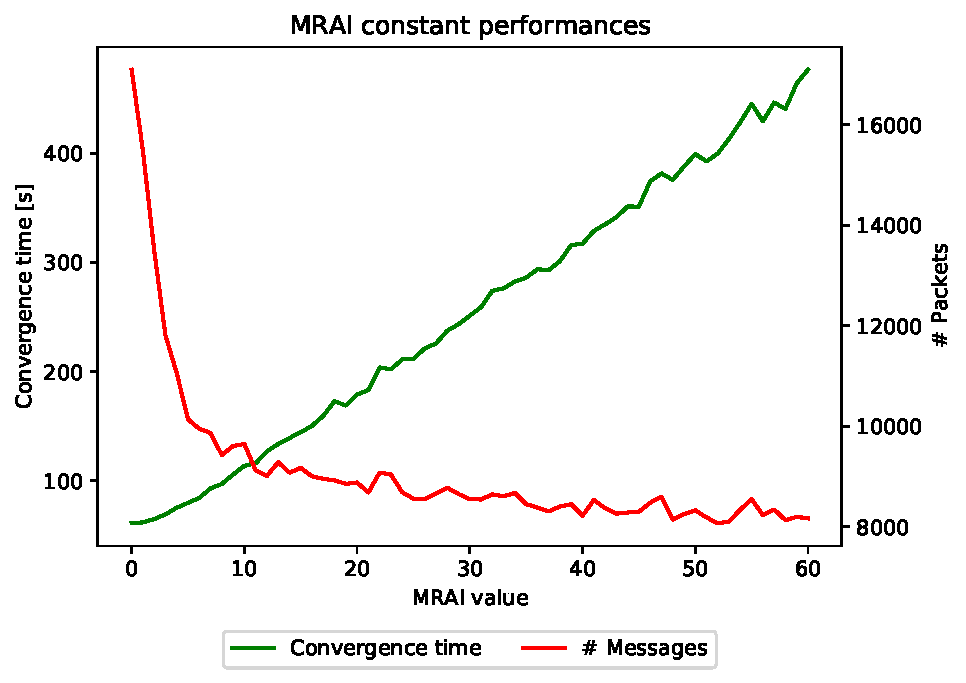
\includegraphics[width=\textwidth]{images/internet_like/1000/constantMRAI/internet_like-constant_mrai_evolution.pdf}
		 \caption{Network performances, messages VS convergence time with different
			\ac{MRAI} values}
         \label{fig:internet_like_1000_constant_evolution_evolution}
     \end{subfigure}
     \hfill
     \begin{subfigure}[b]{0.45\textwidth}
         \centering
         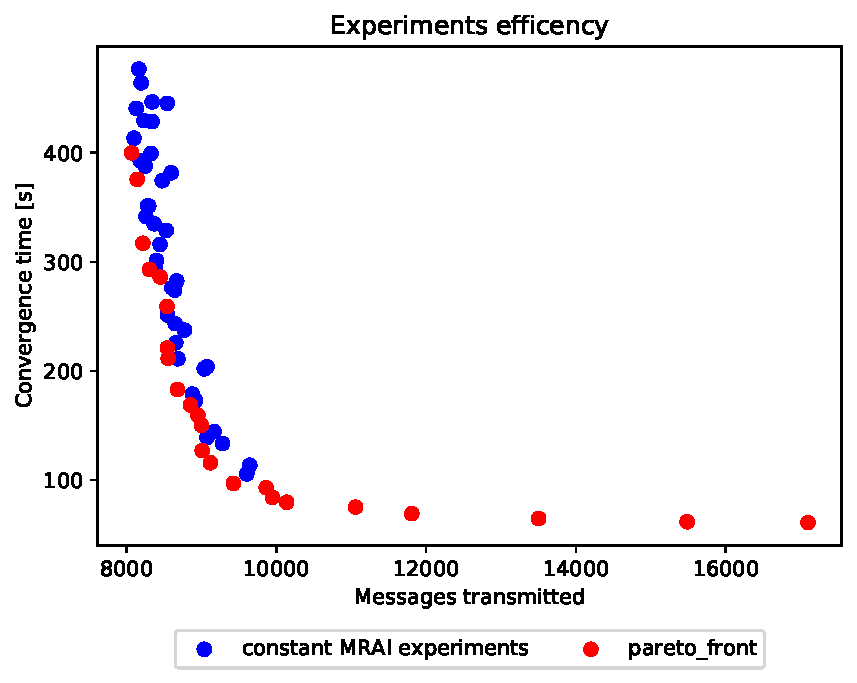
\includegraphics[width=\textwidth]{images/internet_like/1000/constantMRAI/internet_like-constant.pdf}
		 \caption{Pareto front of Messages VS Convergence time}
         \label{fig:internet_like_1000_constant_evolution_paretoFront}
     \end{subfigure}
		\caption{Evolution of the network performances on the \textbf{Internet Like} graph
			of \num{1000} nodes using a fixed \ac{MRAI} from \num{0} to \num{60} seconds.}
        \label{fig:internet_like_1000_constant_evolution}
\end{figure}

As is possible to see in \Cref{fig:internet_like_1000_constant_evolution_evolution}
without \ac{MRAI} we would have a low convergence time, dictated mostly by
network delays and processing time. With, on the other hand, an enormous amount
of messages.
Slightly increasing the \ac{MRAI} value, the number of messages will fell down
reaching a constant value around \num{8000}, while the convergence time
continuously grows linearly, as it happened for the clique graph in \Cref{fig:clique_evolution}.
This continuous linear grow is dictated by the fact that nodes keep meaningful
information for more time before sharing them with their neighbourhood.
\Cref{fig:internet_like_1000_constant_evolution_paretoFront} represent the Pareto
front of those experiments.
The Pareto frontier is the set of values that are Pareto efficient, this concept
has been already used in engineering to define the set of best outcomes from
the trade-off of two different parameters \cite{goodarzi2014introduction}.
We can clearly see that the majority of the points is concentrated on the left
of the chart, this means that few \ac{MRAI} values would give as a result
a high number of messages and a small convergence time.
While multiple \ac{MRAI} values would concentrate around the same value of
messages transmitted.
This can confirm the fact that \ac{MRAI} would not influence messages
after a certain threshold but only the convergence time.

The results of the same environment without \ac{IW} are showed in
\Cref{fig:internet_like_1000_constant_evolution_noIW}.

\begin{figure}[h]
     \centering
     \begin{subfigure}[b]{0.45\textwidth}
         \centering
         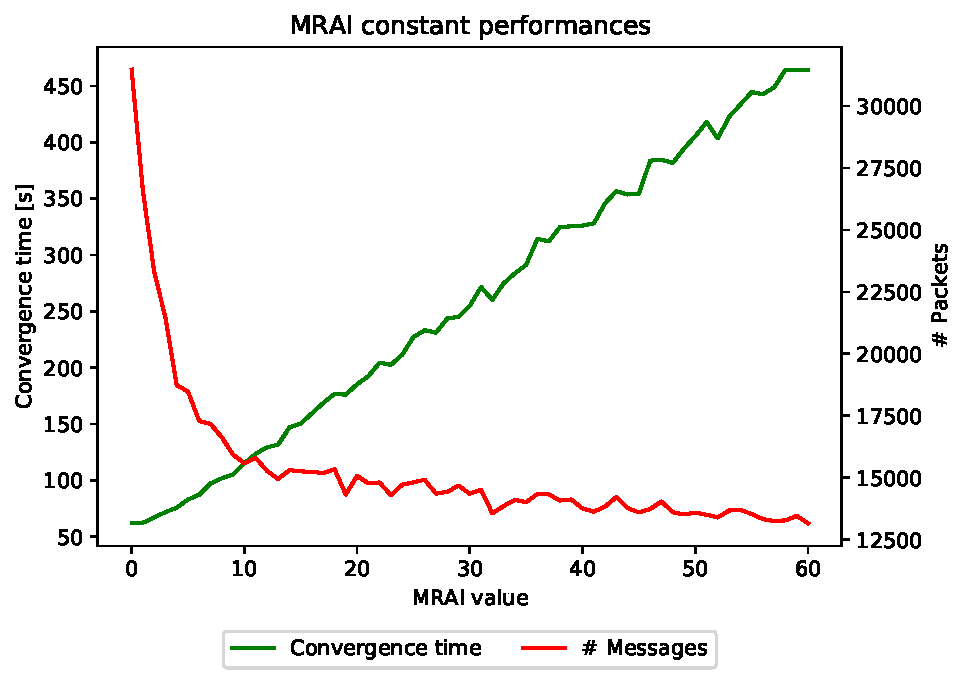
\includegraphics[width=\textwidth]{images/internet_like/1000/constantMRAI/internet_like-constant-noIW_mrai_evolution.pdf}
		 \caption{Network performances, messages VS convergence time with different
			\ac{MRAI} values}
         \label{fig:internt_like_1000_constant_noIW_evolution_evolution}
     \end{subfigure}
     \hfill
     \begin{subfigure}[b]{0.45\textwidth}
         \centering
         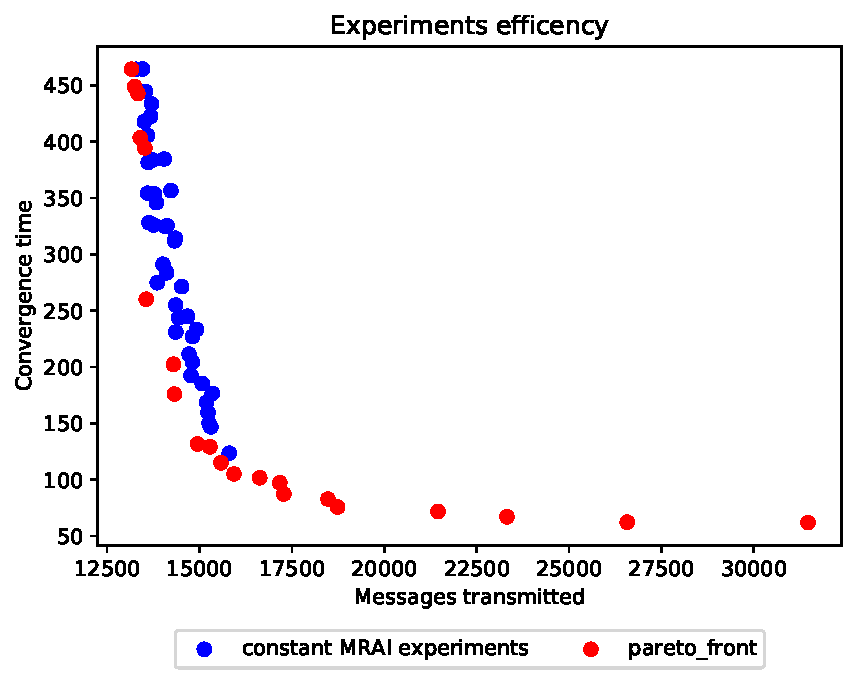
\includegraphics[width=\textwidth]{images/internet_like/1000/constantMRAI/internet_like-constant-noIW.pdf}
		 \caption{Pareto front of Messages VS Convergence time}
         \label{fig:internt_like_1000_constant_noIW_evolution_paretoFront}
     \end{subfigure}
		\caption{Evolution of the network performances on the \textbf{Internet Like} graph
			of \num{1000} nodes using a fixed \ac{MRAI} from \num{0} to \num{60} seconds.
			\textbf{Without \ac{IW}}}
        \label{fig:internet_like_1000_constant_evolution_noIW}
\end{figure}

Also in this case, comparing \Cref{fig:internet_like_1000_constant_evolution_noIW,fig:internet_like_1000_constant_evolution},
is possible to notice that \ac{IW}
helps to reduce the number of messages and the convergence time without impacting
the network performances trend.

The second strategy, the one dependant on the \ac{DPC}, produced the results
in \Cref{fig:internet_like_1000_dpc_evolution}
As mentioned before, all the timers are adjusted to respect the same mean as in
the \textit{fixed} \ac{MRAI} experiments.
For this reason points with the same \ac{MRAI} value are comparable one another.

\begin{figure}[h]
     \centering
     \begin{subfigure}[b]{0.45\textwidth}
         \centering
         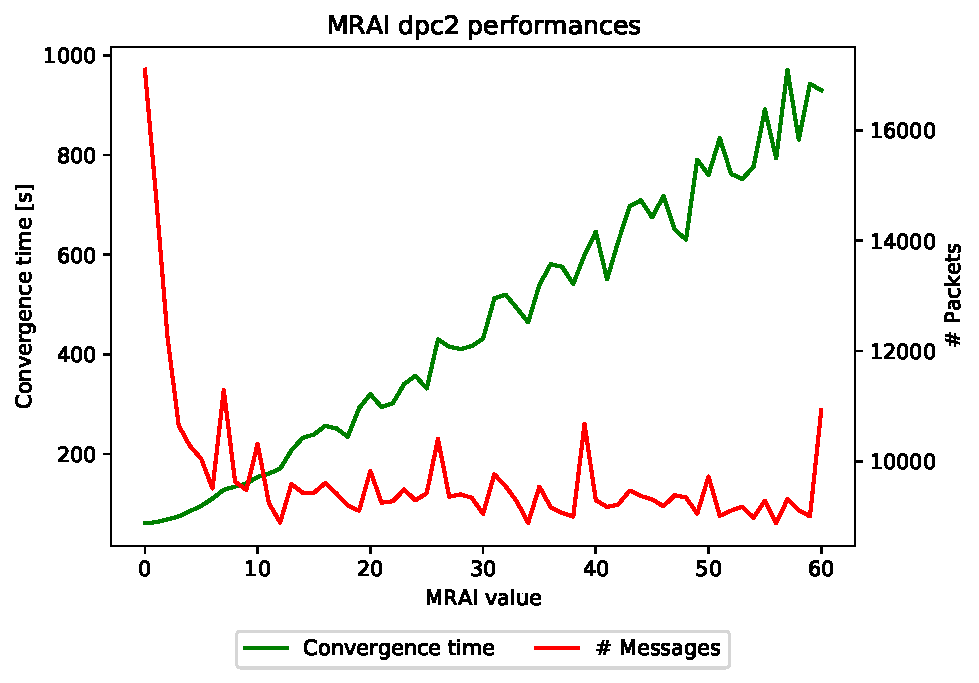
\includegraphics[width=\textwidth]{images/internet_like/1000/dpc/internet_like-DPC_mrai_evolution.pdf}
		 \caption{Network performances, messages VS convergence time with different
			\ac{MRAI} values}
         \label{fig:internt_like_1000_DPC_evolution_evolution}
     \end{subfigure}
     \hfill
     \begin{subfigure}[b]{0.45\textwidth}
         \centering
         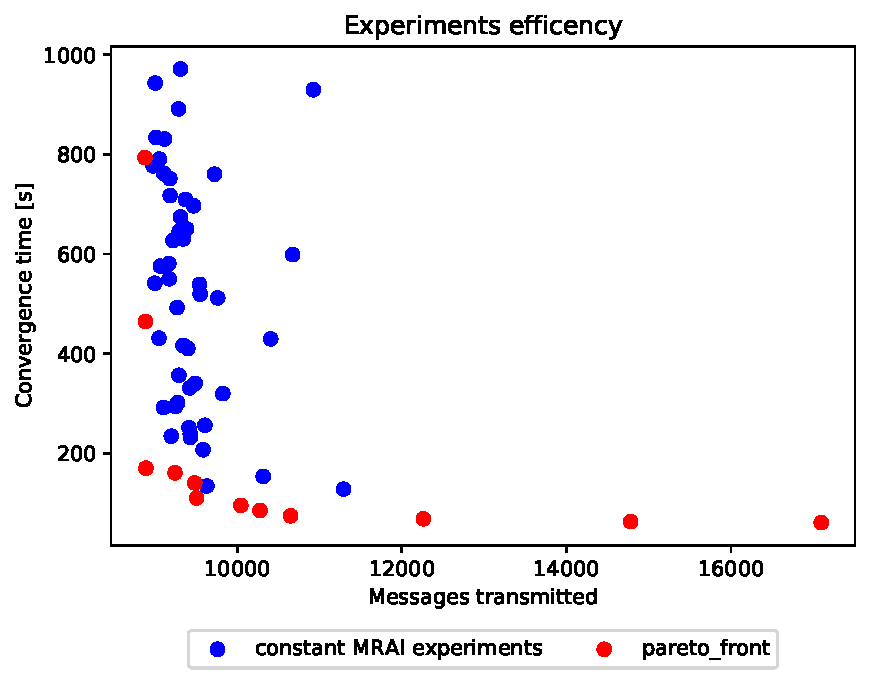
\includegraphics[width=\textwidth]{images/internet_like/1000/dpc/internet_like-DPC.pdf}
		 \caption{Pareto front of Messages VS Convergence time}
         \label{fig:internt_like_1000_DPC_evolution_paretoFront}
     \end{subfigure}
		\caption{Evolution of the network performances on the \textbf{Internet Like} graph
			of \num{1000} nodes using a \textit{DPC} \ac{MRAI} strategy
			with an $MRAI_{mean}$ from \num{0} to \num{60} seconds.}
        \label{fig:internet_like_1000_dpc_evolution}
\end{figure}

This second strategy leads to the performances showed in \Cref{fig:internet_like_1000_dpc_evolution},
where is possible to notice that the number of messages transmitted fell down
very quickly and it reaches the convergence value with an \ac{MRAI} value of
\num{10}.
But, it is also noticeable that there are a lot more spikes in this trend, that
deviate more from the constant value around \num{9000} messages.
And by consequence, the convergence time is affected by this behaviour.

Comparing \Cref{fig:internet_like_1000_dpc_evolution,fig:internet_like_1000_constant_evolution}
is possible to notice that the two strategies lead to a different trend.
Both are equal at the beginning with \ac{MRAI} equal \num{0}, but, after a while,
both the number of transmitted messages and the convergence time diverge.
The number of messages with the \ac{DPC} strategy variate more and it converges
around \num{9000} messages, while the \textit{fixed} strategy reaches \num{8000}
messages.
And the convergence time with the second strategy grows more quickly.
This is caused by the central clique of tier-one nodes that have a high \ac{MRAI}
value.
The high \ac{MRAI} value is caused by the fact that all the leaves has \num{0.0}
as centrality that causes an \ac{MRAI} value of \SI{0}{\second} and to respect
the $MRAI_{mean}$ value the central nodes need a huge \ac{MRAI}.
For example, with an $MRAI_{mean}$ of \SI{30}{\second} the node \num{1} (that is
one of the central clique nodes) has an \ac{MRAI} value of \SI{79.35}{\second} for all its
neighbours.


The standard value of \ac{MRAI} is \SI{30}{\second} as described in
\cite{rfc4271} so I compared those strategies performances in a box-plot in
\Cref{fig:boxplot_internet_like_1000}.
I decided to run \num{100} different runs for each strategy with the $MRAI_{mean}$
fixed to \SI{30}{\second}.

\begin{figure}[h]
     \centering
     \begin{subfigure}[b]{0.45\textwidth}
         \centering
         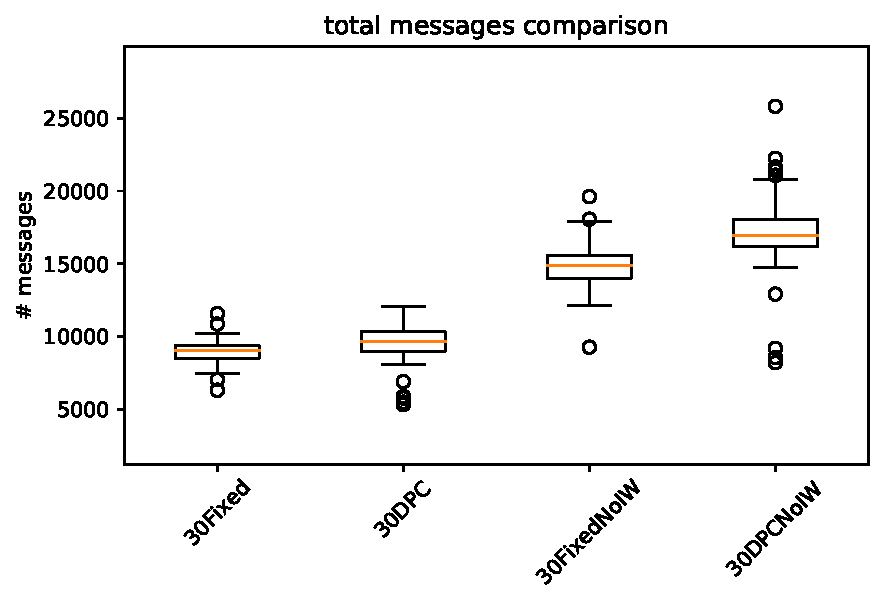
\includegraphics[width=\textwidth]{images/internet_like/1000/comparison/comparison_messages_boxplot.pdf}
		 \caption{Network performances, messages necessary to reach convergence
			with different \ac{MRAI} strategies}
         \label{fig:boxplot_internet_like_1000_messages}
     \end{subfigure}
     \hfill
     \begin{subfigure}[b]{0.45\textwidth}
         \centering
         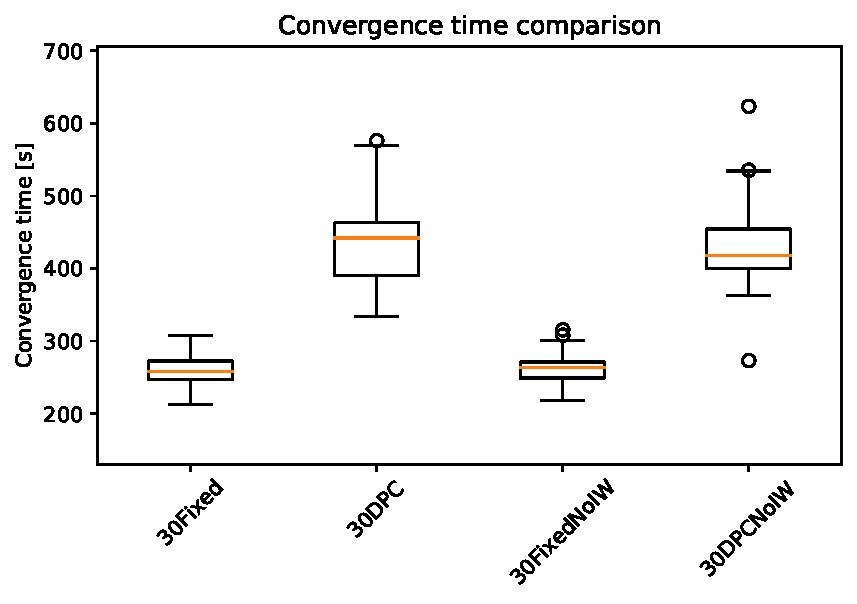
\includegraphics[width=\textwidth]{images/internet_like/1000/comparison/comparison_time_boxplot.pdf}
		 \caption{Network performances, time required to reach convergence
			with different \ac{MRAI} strategies}
         \label{fig:boxplot_internet_like_1000_time}
     \end{subfigure}
	 \caption{Network performances comparison with different \ac{MRAI} strategies,
		Graph internet like with \num{1000} nodes, \ac{MRAI} value
		\SI{30}{\second}, number of runs for each strategy \num{100}}
        \label{fig:boxplot_internet_like_1000}
\end{figure}

In \Cref{fig:boxplot_internet_like_1000} we can compare those two strategies,
the first figure, \Cref{fig:boxplot_internet_like_1000_messages} represent
the number of messages transmitted by the \num{100} runs, we can see that
the two strategies, with the use of \ac{IW}, are really close to one another.
While in the time required for convergence, \Cref{fig:boxplot_internet_like_1000_time},
there are some huge difference between the two strategies, is not negligible
that with the \ac{DPC} strategy the time required is almost the double of the
standard time.

In conclusion, we can say that the \ac{MRAI} strategy is one of the factors that
can influence the Network performances.

\fxfatal{Maybe I can introduce more strategies to expand this section}

\section{Pareto Efficiency Front}
\label{sec:bgp_mrai_pareto_front}

The strategies exposed in \Cref{sec:bgp_mrai_strategy_dependance} are just few
of the available possibilities.
For this reason, I would like to explore the set of possibilities looking
for \ac{MRAI} configuration randomly generated.

I would then study the space of possibilities that are generated through the
Pareto efficiency plot and compare the results with the Pareto efficiency
graphs already presented in \Cref{sec:bgp_mrai_strategy_dependance}.
To permit this comparison I would set \ac{MRAI} randomly but like for
the \ac{DPC} strategy respecting the average required.

The environment used for those experiments is shown in \Cref{tbl:random_env}

\begin{table}[h]
	\begin{center}
	\begin{tabular}{ || m{4.9cm}| m{7.3cm} || } 
	\hline
	Property & Value \\ 
	\hline \hline
	Seeds & $[1, 10]$ \\ 
	\hline
	Signaling & \q{AW} \\
	\hline
		Withdraws delay & Uniform distribution between \SI{1}{\second} and \SI{60}{\second} \\ 
	\hline
		Implicit withdraw & Active \\ 
	\hline
		MRAI mean & $[0, 60]$ \\
	\hline
		MRAI values & Uniform distribution between \SI{1}{\second} and \SI{120}{\second} \\
	\hline
		Experiments per \ac{MRAI} mean & \num{10} \\
	\hline
	Link delay & Uniform distribution between \SI{0.012}{\second} and \SI{3}{\second} \\
	\hline

	\end{tabular}
\end{center}

	\caption{Random \ac{MRAI} environment properties}
	\label{tbl:random_env}
\end{table}

Thanks to this environment I'm going to run in total more than \num{600} complete
experiments.
For each \ac{MRAI} mean value, I will generate \num{10} different graphs with a random
assignment of \ac{MRAI} for each link.
I will then execute \num{10} different runs for each random graph that will produce
the average result of \num{1} experiment.
The total number of experiments is \num{610}.

In \Cref{fig:random_pareto_front} is possible to see all the \num{610} points
generated.

\begin{figure}[h]
    \centering
    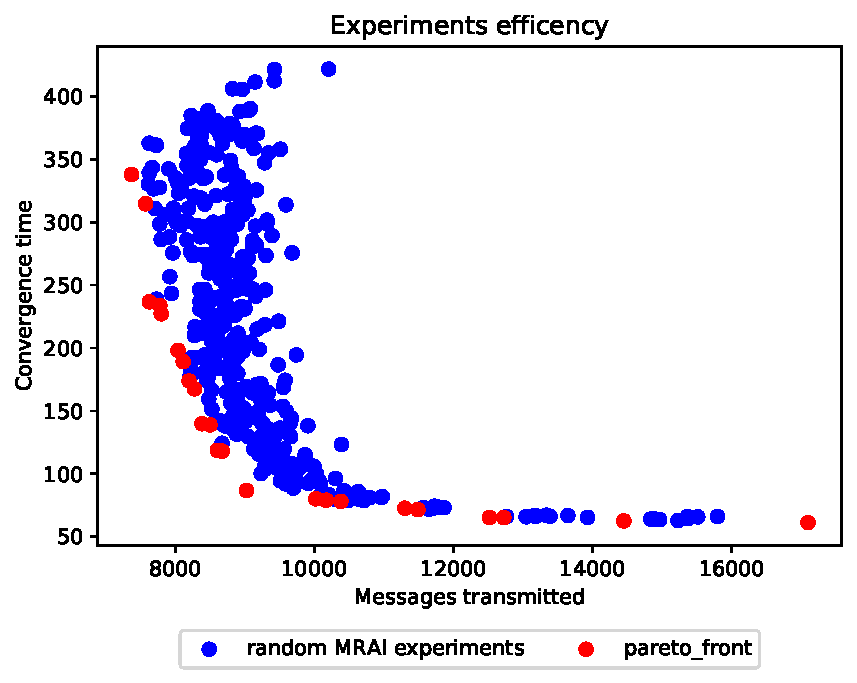
\includegraphics[width=.5\textwidth]{images/internet_like/1000/random.pdf}
	\caption{Pareto front generated by \num{610} experiments on an internet-like
	topology with \num{1000} nodes, \ac{MRAI} generated randomly and adapted to
	the mean \fxfatal{add $[s]$ to the y axis}}
    \label{fig:random_pareto_front}
\end{figure}

As we can see the trend in \Cref{fig:random_pareto_front} is similar to the one
that we saw for the same signal in \Cref{sec:bgp_mrai_strategy_dependance}.
For the majority of configurations, the number of messages transmitted is never
over \num{10000} but the time required to converge grows continuously.

In \Cref{fig:pareto_comparison} is present a comparison between the random
experiments, the fixed \ac{MRAI} strategy and the \ac{DPC} strategy from
\Cref{fig:internet_like_1000_constant_evolution_paretoFront,fig:internt_like_1000_DPC_evolution_paretoFront}

\begin{figure}[h]
    \centering
    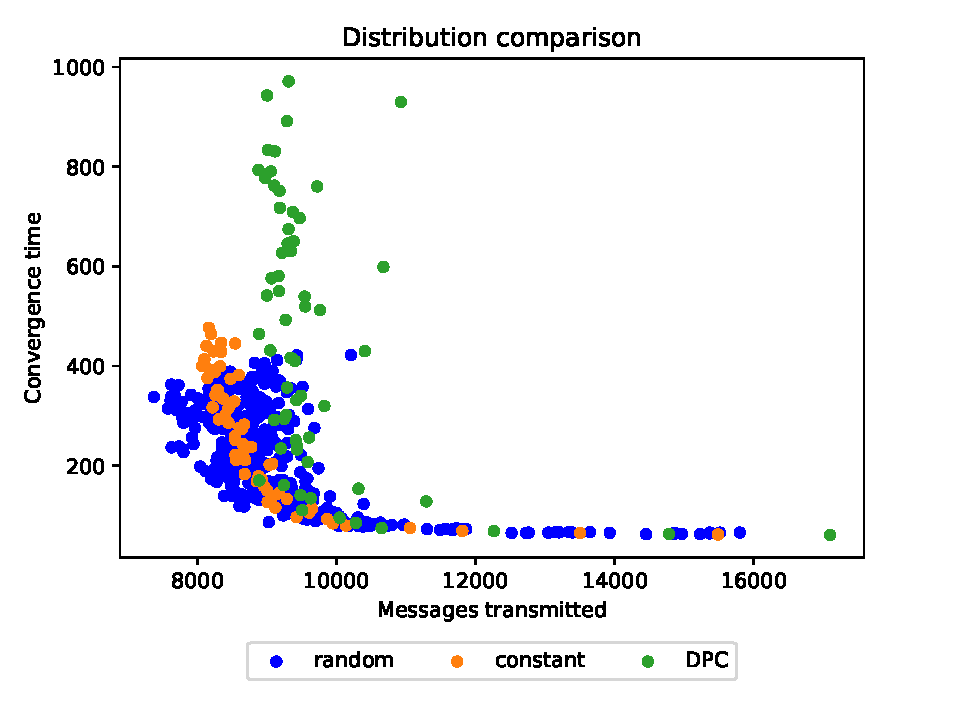
\includegraphics[width=.57\textwidth]{images/internet_like/1000/random_vs_all.pdf}
	\caption{Pareto front generated by \num{601} experiments on an internet-like
	topology with \num{1000} nodes, \ac{MRAI} generated randomly and adapted to
	the mean, vs fixed \ac{MRAI} strategy and \ac{DPC} \ac{MRAI} strategy.
	\fxfatal{add $[s]$ to the y axis}}
    \label{fig:pareto_comparison}
\end{figure}

As we can see in \Cref{fig:pareto_comparison} all the strategies have the same
behaviour, but is also possible to see that the random strategy is the only
one with experiments that produce less than \num{8000} messages.
This is important because its a proof that there are better possibilities rather
that the classical one.

For this reason, \ac{MRAI} can be tuned to have a better trade-off between
the number of messages transmitted and convergence time.

\section{Signal dependence}
\label{sec:bgp_mrai_signal_dependance}

I would like to analyze how much the signal can impact the convergence performances
with the two different strategies of \Cref{sec:bgp_mrai_strategy_dependance}.

For this reason, I used the same environment described before and execute the
experiments with different input signals from the same node, \q{AWA}, \q{AWAW}
and \q{AWAWA}.

In those experiments plays a role also the \q{\textit{re-advertisement distribution}}
for the second and third \q{A}, it has been set to a uniform distribution
between \SI{1}{\second} and \SI{60}{\second}, like the \q{\textit{withdraw distribution}}.

For those experiments, I didn't evaluate the case with \ac{IW} deactivated.
Because, like we saw in,
\Cref{fig:internet_like_1000_constant_evolution,fig:internet_like_1000_constant_evolution_noIW}
there is not a difference in terms of the trend but only on the number of messages
transmitted.
So we can easily imagine that the performance of the following experiments
wouldn't have other big differences, except for the number of messages, with the
\ac{IW} active.

\fxfatal{all the plots has an \ac{MRAI} steep of \SI{10}{\second} to give a
hint on the trend, redo the plots with a step of \SI{1}{\second}}

In \Cref{fig:internt_like_1000_evolution_AWA} is possible to see the evolution
for the signal \q{AWA}.

\begin{figure}[h]
     \centering
     \begin{subfigure}[b]{0.45\textwidth}
         \centering
         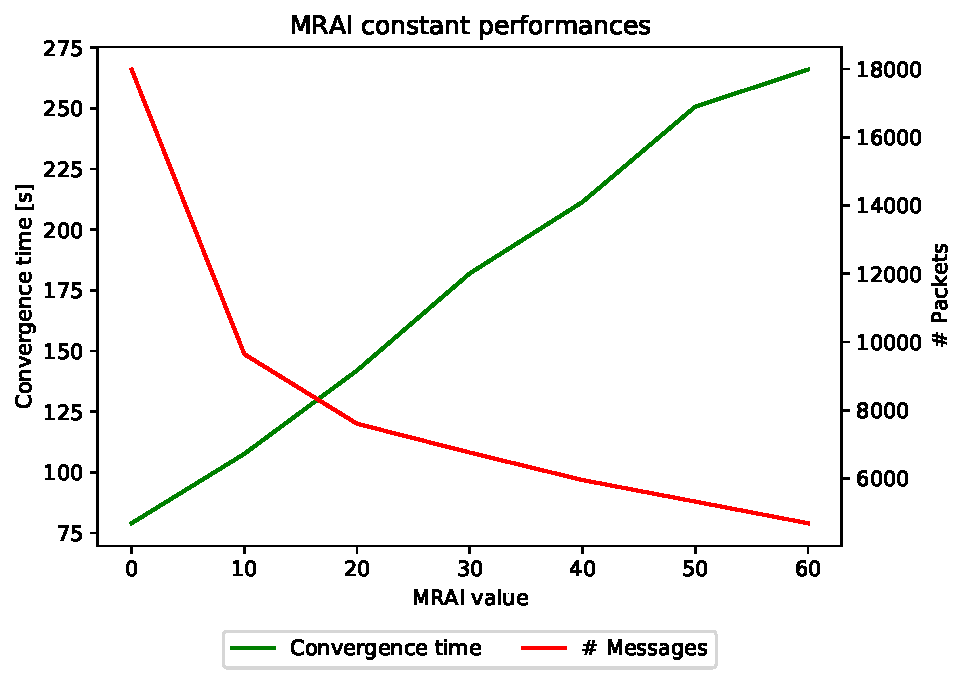
\includegraphics[width=\textwidth]{images/internet_like/1000/signals/AWA/constant/internet_like-constant_AWA_mrai_evolution.pdf}
		 \caption{Network performances, \textit{fixed} \ac{MRAI} strategy}
         \label{fig:internet_like_1000_fixed_AWA}
     \end{subfigure}
     \hfill
     \begin{subfigure}[b]{0.45\textwidth}
         \centering
         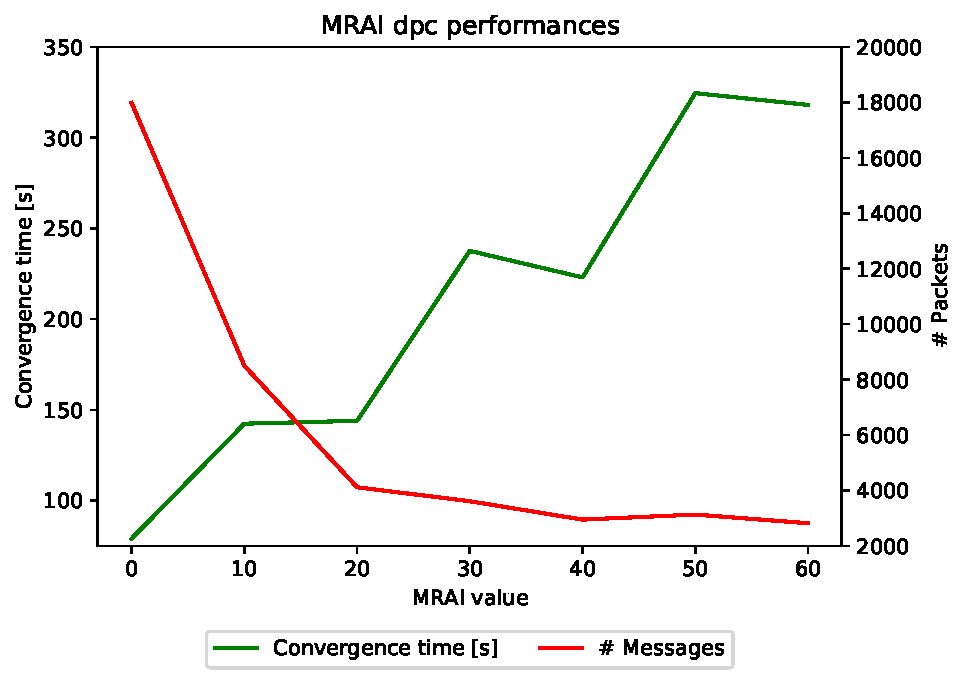
\includegraphics[width=\textwidth]{images/internet_like/1000/signals/AWA/dpc/internet_like-DPC_AWA_mrai_evolution.pdf}
		 \caption{Network performances, \ac{DPC} \ac{MRAI} strategy}
         \label{fig:internet_like_1000_dpc_AWA}
     \end{subfigure}
	 \caption{Network performances comparison with different \ac{MRAI} strategies,
		Graph internet like with \num{1000} nodes, signal \q{AWA}}
        \label{fig:internt_like_1000_evolution_AWA}
\end{figure}

Is possible to notice in \Cref{fig:internt_like_1000_evolution_AWA} a huge difference
in respect of the plots in \Cref{fig:internet_like_1000_constant_evolution,fig:internet_like_1000_dpc_evolution}.
The \ac{DPC} strategy was able to outcome the standard \textit{fixed} strategy
over multiple prospective.
Analyzing \Cref{fig:internet_like_1000_dpc_AWA} is possible to notice that
the red curve, the one that refers to the number of messages transmitted has
a very fast fell, with an average \ac{MRAI} timer \textit{of \SI{30}{\second}}
the number of messages is less than $1/4$ in respect of an \ac{MRAI} \textit{mean}
of \SI{0}{\second}.
The convergence time curve has a completely different trend in respect of the
previous experiments.
We can notice some steps trend.
This is caused by the fact that now the timer is able to effectively act on the signal.
\ac{MRAI} doesn't affect the first message, in this case, the first \q{A} of the
signal, but it can affect the next two messages.
In fact, some nodes are able to cache both the \q{WA} part of the signal and
completely avoid sending anything at all, because they have already transmitted
the first \q{A}.
The complete compression of the signal \q{AWA} is \q{A}.
The other evolution, for the \q{AWAW} and \q{AWAWA} signals, are showed in
\Cref{fig:internt_like_1000_evolution_AWAW,fig:internt_like_1000_evolution_AWAWA}

Like before, comparing the standard \SI{30}{\second} fixed \ac{MRAI} I executed
\num{100} different runs for each strategy and each different signal, the results
are showed in \Cref{fig:boxplot_internet_like_1000_time_allSignals}.

\begin{figure}[h]
     \centering
     \begin{subfigure}[b]{0.45\textwidth}
         \centering
         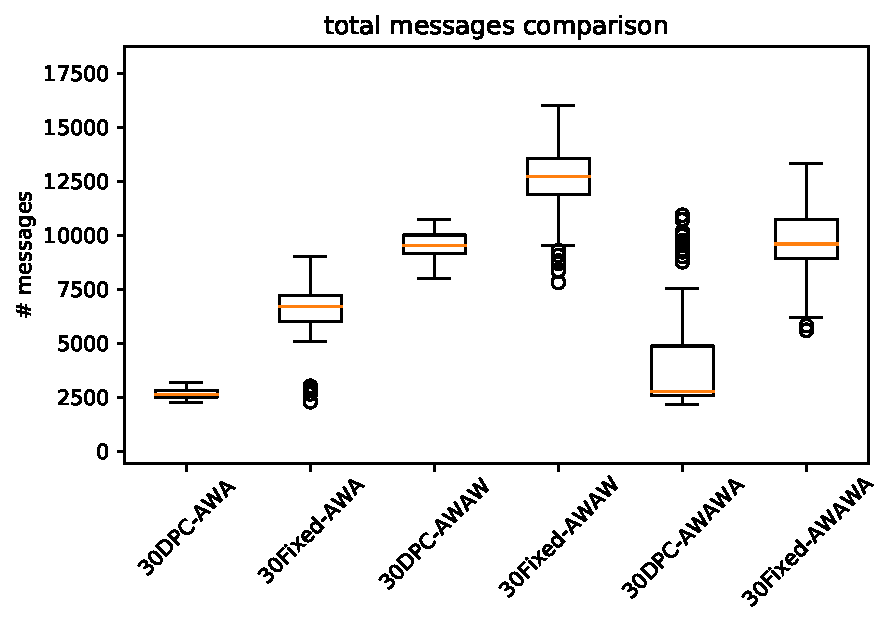
\includegraphics[width=\textwidth]{images/internet_like/1000/comparison/comparison_allSignals_messages_boxplot.pdf}
		 \caption{Network performances, messages necessary to reach convergence
			with different \ac{MRAI} strategies}
         \label{fig:boxplot_internet_like_1000_messages_allSignals}
     \end{subfigure}
     \hfill
     \begin{subfigure}[b]{0.45\textwidth}
         \centering
         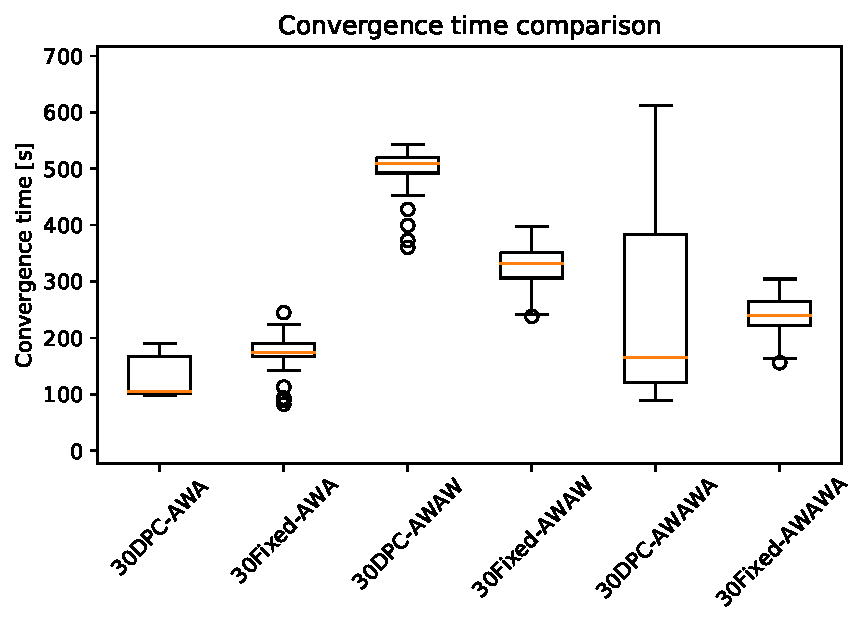
\includegraphics[width=\textwidth]{images/internet_like/1000/comparison/comparison_allSignals_time_boxplot.pdf}
		 \caption{Network performances, time required to reach convergence
			with different \ac{MRAI} strategies}
         \label{fig:boxplot_internet_like_1000_time_allSignals}
     \end{subfigure}
	 \caption{Network performances comparison with different \ac{MRAI} strategies,
		Graph internet like with \num{1000} nodes, \ac{MRAI} value
		\SI{30}{\second}, number of runs for each strategy \num{100}, signal \q{allSignals}}
        \label{fig:boxplot_internet_like_1000_allSignals}
\end{figure}

Is possible to notice in \Cref{fig:boxplot_internet_like_1000_allSignals} that
both the strategies have different performances in respect of the signal
produced by the single node source.
In particular, performances are better when the signal ends up with an \q{A}.
That's because, after the first \q{A}, giving a \ac{MRAI} timer long enough,
a node is able to compress a sequence that ends with another \q{A} to the
empty set and don't send anything more.
While if the sequence ends up with an \q{W} it has to, at least, send another
message to notify the withdraw.

Other than that is possible to notice that the \ac{DPC} techniques have better
results in terms of messages transmitted, while it could have a higher
convergence time.
This is caused, like before, by the high \ac{MRAI} values used by the most
central nodes.

In conclusion, there is a correlation between \ac{MRAI} and the sequence of messages
transmitted by the source node.
In particular more the timer is able to compress the sequence more the performances
can be improved.

\section{Position dependence}
\label{sec:position_dependance}

The last factor of influence for \ac{MRAI} that I would like to study is how much
the position of the signal source can influence the convergence.
The main hypothesis is that a node closer to the central clique, that generates
a signal would provoke a message storm bigger in respect of a node on the perimeter
of the network.
This is true only if \ac{MRAI} is large enough to block the storm near the source
of it exporting only the correct information at the end of it.

\subsection{Different signal sources}
\label{subsec:different_destinations}

As first try I have decided to analyse \num{10} different destination chosen randomly
on the same graph, this graph is an Internet like topology with \num{1000} nodes.
After that, I run the same environment with all the different destination.
I also used different \ac{MRAI} strategies, repeating the experiments for all of
them.
With this results is possible to analyze how different signal sources provoke
different network performances and also study how different \ac{MRAI} strategies
adapt to different nodes that provoke messages storms.

The environment used by those experiments is the one described in
\Cref{tbl:source_properties}.

\begin{table}[h]
	\begin{center}
	\begin{tabular}{ || m{4cm}| m{8cm} || }
	\hline
	Property & Value \\
	\hline \hline
	Seeds & $[1, 10]$ \\
	\hline
	Signaling & \q{AWAWA} \\
	\hline
		Withdraws delay & Uniform distribution between \SI{0.1}{\second} and \SI{60}{\second} \\
	\hline
	Announcement delay & Uniform distribution between \SI{0.1}{\second} and \SI{60}{\second} \\
	\hline
	Link delay & Uniform distribution between \SI{0.0001}{\second} and \SI{0.5}{\second} \\
	\hline
			\(MRAI_{mean}\) & $[0, 60]$ with steps of \num{10} \\
	\hline
		Random nodes & \num{10} \\
	\hline
		\ac{MRAI} strategies & Fixed \ac{MRAI}, \ac{DPC}, reverse \ac{DPC} \\
	\hline
	\end{tabular}
\end{center}

	\caption{Different signal sources environment properties}
	\label{tbl:source_properties}
\end{table}

Like mentioned in \Cref{tbl:source_properties} I decided to use another
\ac{MRAI} strategy and look forward to its performances.
That strategy is the reverse of the one base on the \ac{DPC}.
I will use a higher \ac{MRAI} for the first part of the graph and a smaller
one in the propagation part of the graph.

In total, I have executed \num{700} runs for each \ac{MRAI} strategy with the
\num{10} different signal sources.
The resulting network evolution with different \ac{MRAI} values is shown in
\Cref{fig:different_destinations}.
Each point of \Cref{fig:different_destinations_all} represents the average
of the \num{10} runs executed for the specific destination with that \ac{MRAI}
configuration.
On \Cref{fig:different_destinations_mean} is presented the average result
obtained from all the \num{10} different destinations for a specific \ac{MRAI}
strategy.

\begin{figure}[h]
     \centering
     \begin{subfigure}[b]{0.45\textwidth}
         \centering
         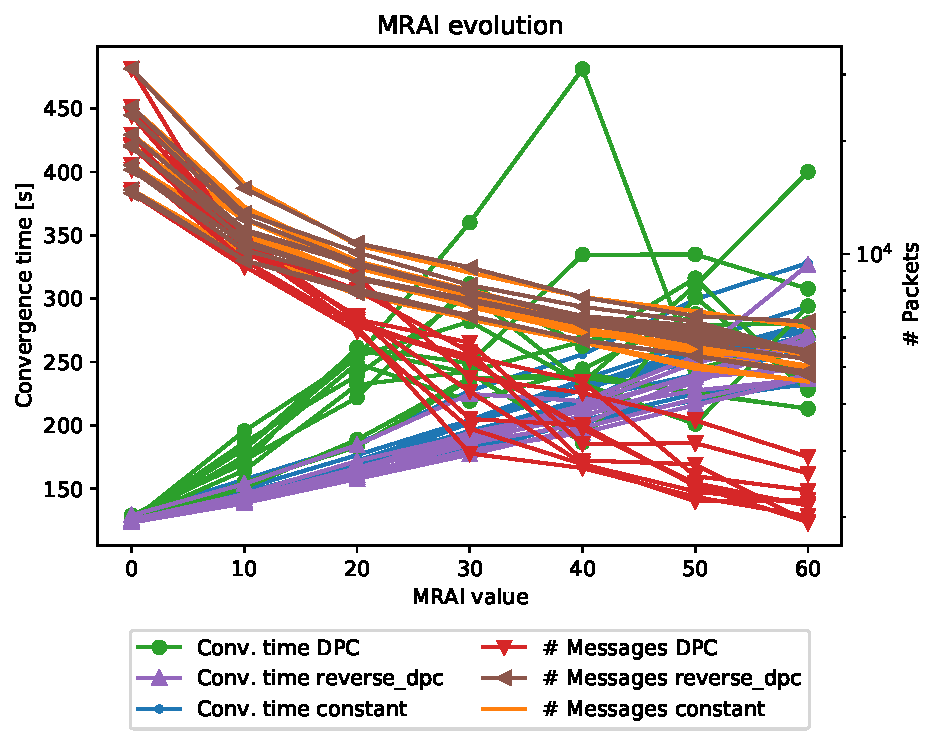
\includegraphics[width=\textwidth]{images/position/different_destinations-1000_all.pdf}
		 \caption{Network performance evolution of all the \num{10} different signal sources
			with the different \ac{MRAI} strategies}
         \label{fig:different_destinations_all}
     \end{subfigure}
     \hfill
     \begin{subfigure}[b]{0.45\textwidth}
         \centering
         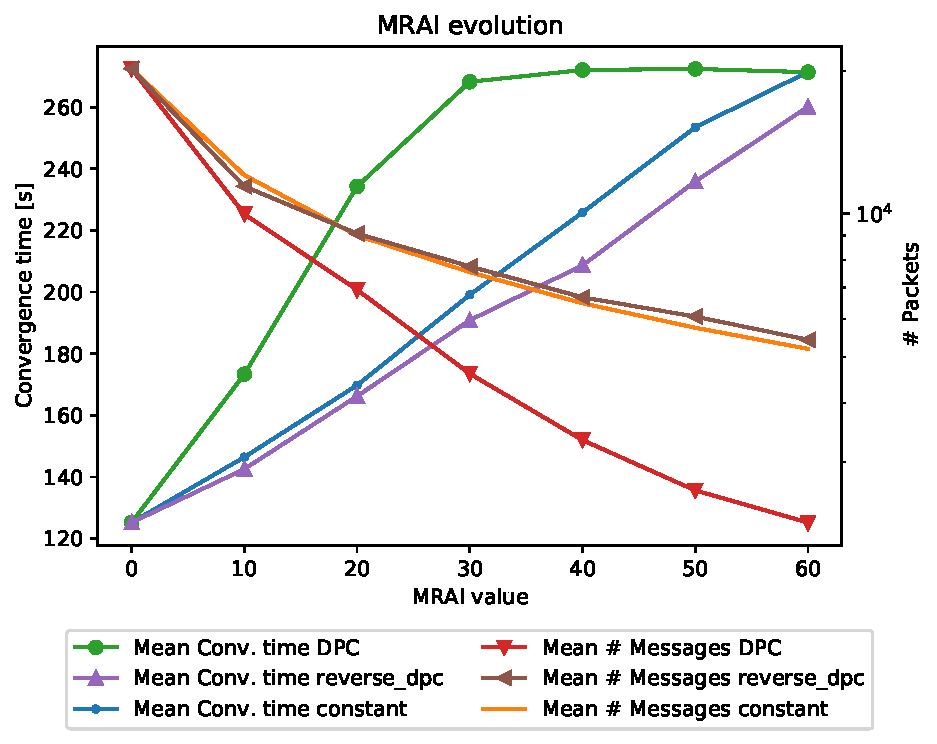
\includegraphics[width=\textwidth]{images/position/different_destinations-1000_mean.pdf}
		 \caption{Average of the network performances of \num{10} different
			signal sources are chosen with different \ac{MRAI} strategies}
         \label{fig:different_destinations_mean}
     \end{subfigure}
	 \caption{Network performances given \num{10} different signal sources chosen
		randomly on an Internet like graph of \num{1000} nodes, with different
		\ac{MRAI} strategies used, fixed, \ac{DPC}, Reverse \ac{DPC}, and
		different \ac{MRAI} mean values}
	 \label{fig:different_destinations}
\end{figure}

\Cref{fig:different_destinations} shows how, changing the source of the signal,
also changes the network performances with multiple \ac{MRAI} values.
Notice that the second y-axis, the one that represents the number of packets
transmitted, is in log scale.
We can use the plot in \Cref{fig:different_destinations_all} to see the
differences between one destination and the others, while \Cref{fig:different_destinations_mean}
expose the differences between different strategies.
We can see in \Cref{fig:different_destinations_all} that all the \num{10} destinations
cause a similar behaviour with the fixed strategy and the reverse \ac{DPC}, both
in terms of messages transmitted and also convergence time.
In both techniques, the difference between the \num{10} destinations in terms of
convergence time is a few tens of seconds, with linear growth.
Thanks to \Cref{fig:different_destinations_mean} is possible to see that the
number of messages reaches a convergence value around between \num{5000} and
\num{6000}.
The \ac{DPC} strategy seems to bee more volatile with the growth of \ac{MRAI}
both in terms of messages and also convergence time.
We can clearly see from multiple green spikes in \Cref{fig:different_destinations_all}
that the position of the source is highly affective using this strategy.

\fxfatal{Consider using a table to show the average and the std var of conv time
and messages}

We can conclude that the position of the source can influence the behaviour
of \ac{MRAI}, it is more influenced when the strategy used relies on topological
information, like the \ac{DPC} strategy.

\subsection{Hierarchical influence}
\label{subsec:hierarchical_influence}

What about the position in the hierarchy?
Internet is very strong hierarchical graph, \Cref{fig:internet_topology_hierarchical}
is an example with a small set of nodes but it is possible to define different levels
of the graph.
If we take the central clique as the root of the graph then all the nodes will
be at a certain distance (in terms of hops) from it.

Nodes that are on the same hierarchical level reacts in the same way?

To analyze this possibility I decided to take \num{3} nodes randomly from each
hierarchical level of an Internet-like graph of \num{1000} nodes, the number
of levels on this graph was \num{4}.
The total number of destinations was \num{12} and for each one of them I executed
an experiment with multiple \ac{MRAI} strategies and multiple possible \ac{MRAI}
values.

The properties of this environment are summarized in \Cref{tbl:hierarchical_properties}.

\begin{table}[h]
	\begin{center}
	\begin{tabular}{ || m{4cm}| m{8cm} || } 
	\hline
	Property & Value \\ 
	\hline \hline
	Seeds & $[1, 10]$ \\ 
	\hline
	Signaling & \q{AWAWAWAW} \\
	\hline
		Withdraws delay & Uniform distribution between \SI{0.1}{\second} and \SI{5}{\second} \\ 
	\hline
	Announcement delay & Uniform distribution between \SI{0.1}{\second} and \SI{5}{\second} \\ 
	\hline
	Link delay & Uniform distribution between \SI{0.0001}{\second} and \SI{0.5}{\second} \\
	\hline
		MRAI & $[0, 60]$ with steps of \num{10} \\
	\hline
		Number of levels & \num{4} \\
	\hline
		Random dst per level & \num{3} \\
	\hline
		\ac{MRAI} strategies & \ac{DPC}, reverse \ac{DPC} \\
	\hline
	\end{tabular}
\end{center}

	\caption{Hierarchical experiments environment properties}
	\label{tbl:hierarchical_properties}
\end{table}

Given that we are evaluating the impact of nodes by their distance from
the center of the network, it could be a good way also to test strategies
which goal is to enforce those points, for this reason, I chose those two
strategies.

The results in \Cref{fig:different_levels} shows the different evolution of
the random source for each different level, from the first to the fourth.

\begin{figure}[h]
     \centering
     \begin{subfigure}[b]{0.45\textwidth}
         \centering
         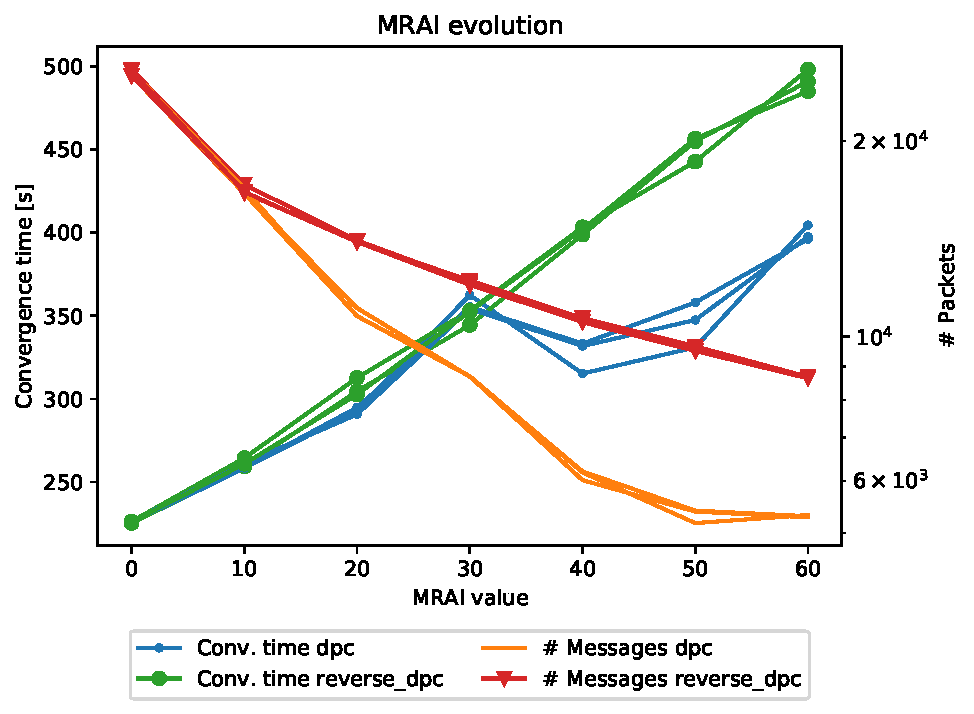
\includegraphics[width=\textwidth]{images/hierarchy/different_levels-1000_hier_1_all.pdf}
		 \caption{Network performances evolution of all the \num{3} different signal sources
			with the different \ac{MRAI} strategies at the hierarchical level \num{1}}
         \label{fig:different_levels_1}
     \end{subfigure}
     \begin{subfigure}[b]{0.45\textwidth}
         \centering
         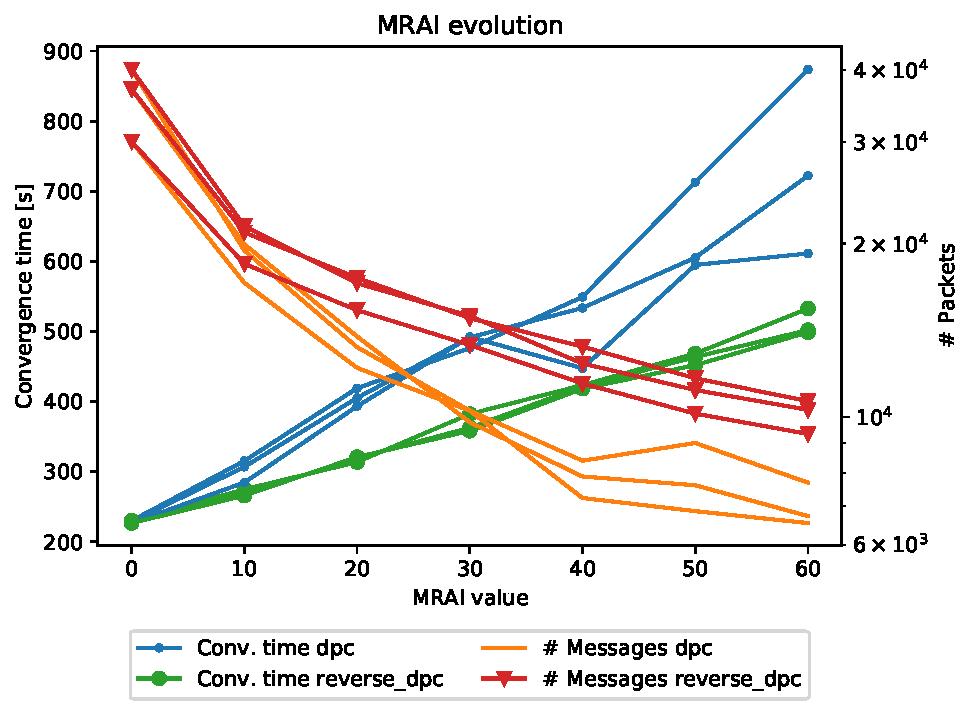
\includegraphics[width=\textwidth]{images/hierarchy/different_levels-1000_hier_2_all.pdf}
		 \caption{Network performances evolution of all the \num{3} different signal sources
			with the different \ac{MRAI} strategies at the hierarchical level \num{2}}
         \label{fig:different_levels_2}
     \end{subfigure}
     \begin{subfigure}[b]{0.45\textwidth}
         \centering
         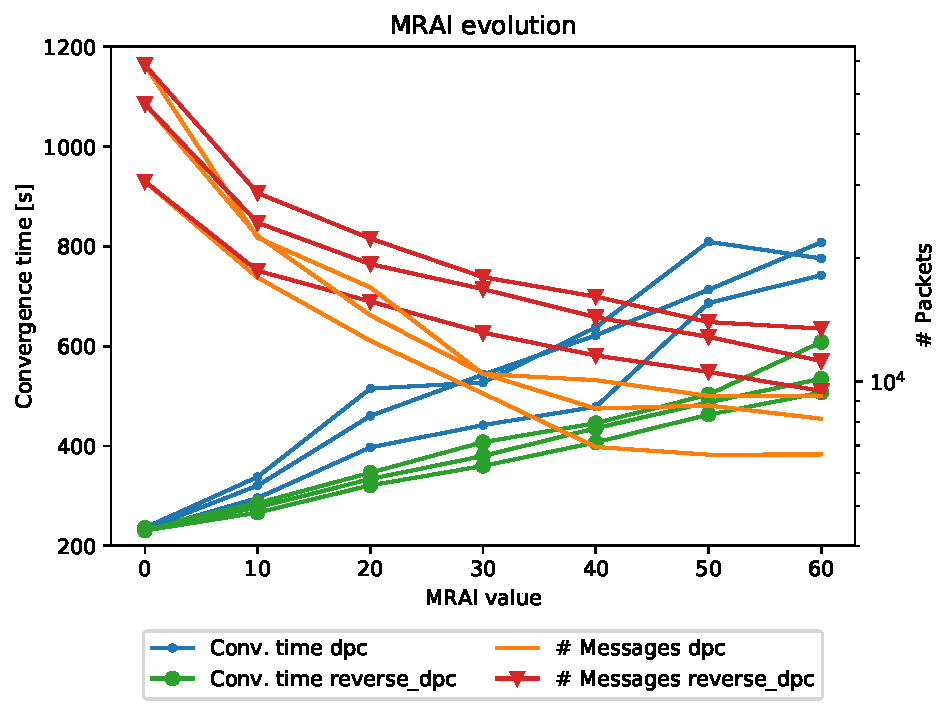
\includegraphics[width=\textwidth]{images/hierarchy/different_levels-1000_hier_3_all.pdf}
		 \caption{Network performances evolution of all the \num{3} different signal sources
			with the different \ac{MRAI} strategies at the hierarchical level \num{3}}
         \label{fig:different_levels_3}
     \end{subfigure}
     \begin{subfigure}[b]{0.45\textwidth}
         \centering
         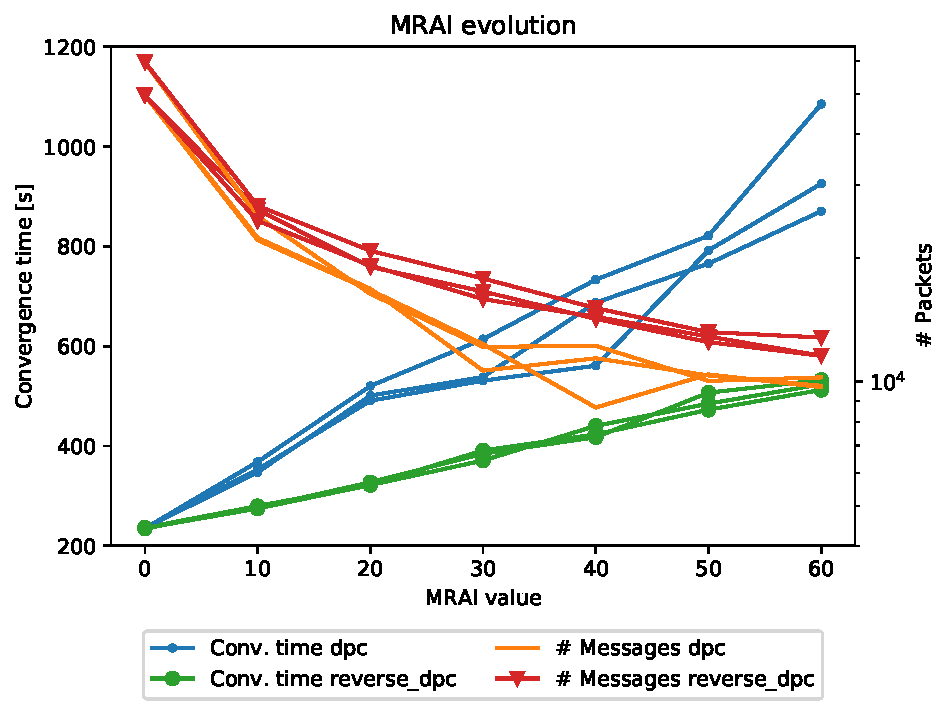
\includegraphics[width=\textwidth]{images/hierarchy/different_levels-1000_hier_4_all.pdf}
		 \caption{Network performances evolution of all the \num{3} different signal sources
			with the different \ac{MRAI} strategies at the hierarchical level \num{4}}
         \label{fig:different_levels_4}
     \end{subfigure}
     \hfill
	 \caption{Network performances given \num{3} different signal sources chosen
		randomly for each level of the Internet like graph, number of nodes
		\num{1000}, number of levels \num{4}, different \ac{MRAI} strategies
		\ac{DPC} and reverse \ac{DPC} \fxfatal{Adjust messages ticks}}
	 \label{fig:different_levels}
\end{figure}

In \Cref{fig:different_levels} is possible to see the evolution of the network
with different source nodes from different levels and how \ac{MRAI} influence
the network performances.
Starting from the first level in \Cref{fig:different_levels_1}, where the source
node was directly connected with a node of the central clique we can see different
important things.
First of all, the variance that the three different sources have is very small,
both in terms of messages transmitted and also convergence time.
Both the techniques, \ac{DPC} and the reverse of it, in terms of messages
transmitted starts from a value around \num{25000} with \ac{MRAI} equal to
\SI{0}{\second} and both reaches a value under \num{10000} units.
In terms of convergence time, the reverse strategy grows linearly as expected
while the \ac{DPC} technique is able to gain a strong reduction thanks to
the efficient messages compression.
Going to the second and third level, respectively in
\Cref{fig:different_levels_2,fig:different_levels_3} when can see that there
is an increase of the variance between the single source trends, both in terms
of messages and also convergence time.
Also, the number of messages transmitted slowly increases, at the beginning the
number of messages reaches \num{60000} units converging around \num{10000}.
In \Cref{fig:different_levels_3} we can see the worst-case scenario, not in
terms of variance between the sources, but in this case, we have the worst
performances.
The convergence time grows even over \SI{1000}{\second} for the \ac{DPC} strategy.
While the number of messages transmitted with \ac{MRAI} equal to \SI{0}{\second}
touches \num{60000} reaching a convergence value slightly over \num{10000}.

We can clearly see the influence that the position of the source nodes has to
a hierarchical graph like the Internet.
The performances with \ac{MRAI} at \SI{0}{\second} are only attributable to the
strategic position of the source node.

Another hypothesis is that there is a difference in the single nodes based
on the position in the topology.
Nodes that are more central, if the signal comes from closer nodes could
react with a more explosive \textit{Path exploration} behaviour.
If the signal comes from the periphery of the network, the other side of
it could require more time to converge in respect of a signal that starts
near the center.

To prove that hypothesis I decided to use the data from this set of experiments
with \ac{MRAI} value equal to \SI{30}{\second}.
I calculated for each node the average performances, based on the level, convergence
time, number of messages necessary to reach the convergence state and \ac{DPC}
centrality value (that is dependant on the position of the source).
I have then grouped nodes that are at the same distance from the source, to
calculate the distance I used the distance in terms of hops in the \textit{Best
Path}.
I then calculated the average performances of each group.
The results are showed in \Cref{fig:different_levels_comparison}.

\begin{figure}[h]
     \centering
     \begin{subfigure}[b]{0.45\textwidth}
         \centering
         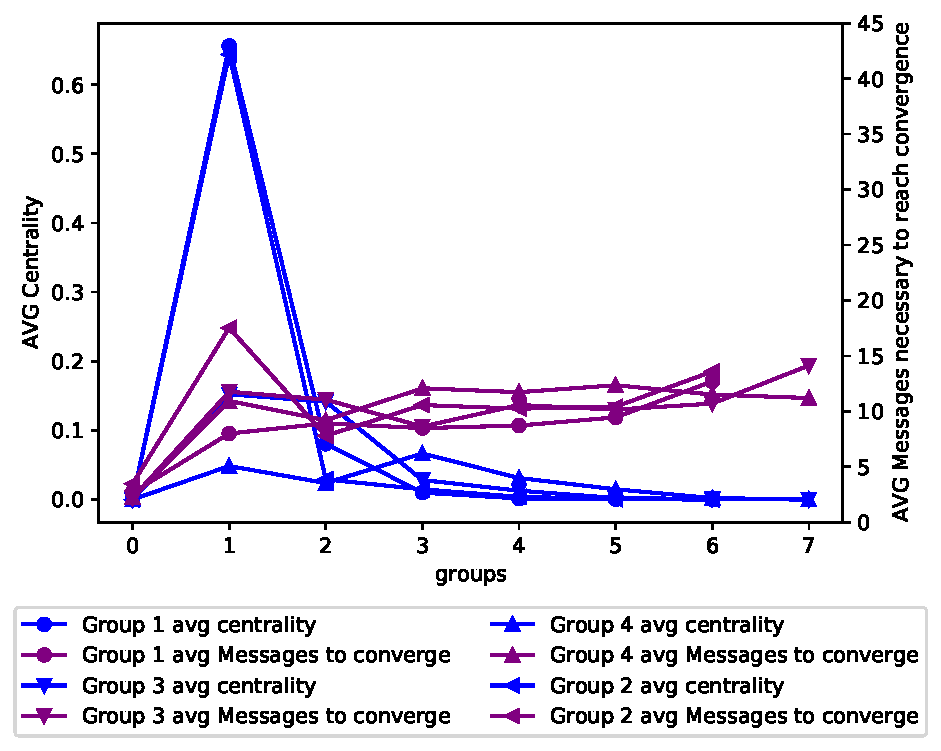
\includegraphics[width=\textwidth]{images/hierarchy/dpc_all_levels_comparison_centVSmsg.pdf}
		 \caption{\ac{MRAI} strategy \ac{DPC}, number of messages necessary on
			average to reach convergence, levels comparison}
         \label{fig:different_levels_comparison_dpc_msg}
     \end{subfigure}
     \begin{subfigure}[b]{0.45\textwidth}
         \centering
         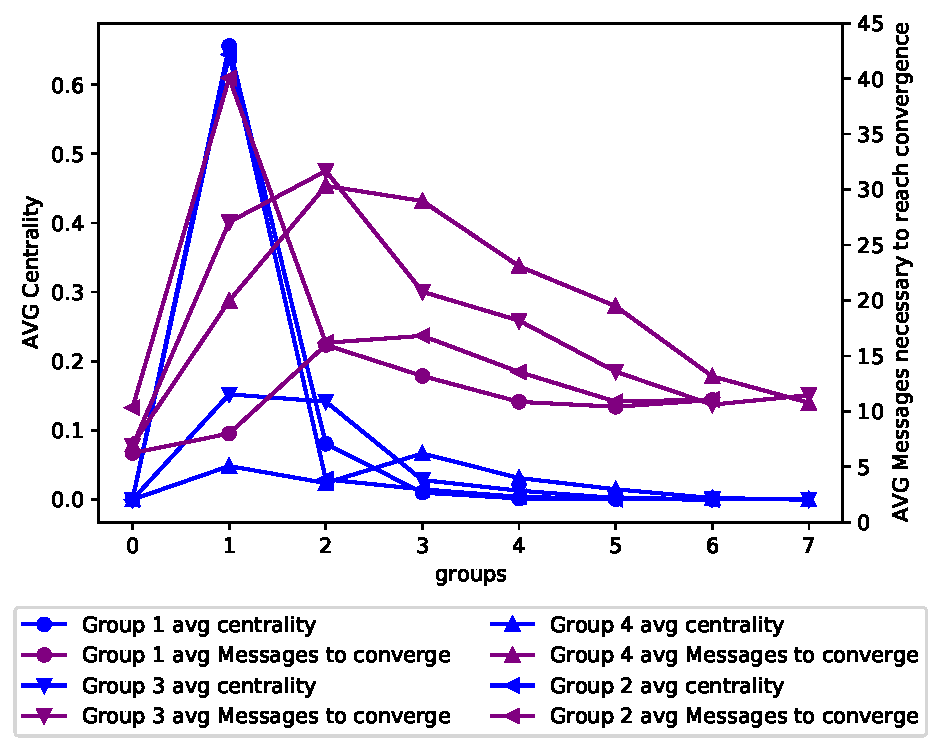
\includegraphics[width=\textwidth]{images/hierarchy/reverse_dpc_all_levels_comparison_centVSmsg.pdf}
		 \caption{\ac{MRAI} strategy reverse \ac{DPC}, number of messages necessary on
			average to reach convergence, levels comparison}
         \label{fig:different_levels_comparison_reverse_dpc_msg}
     \end{subfigure}
     \begin{subfigure}[b]{0.45\textwidth}
         \centering
         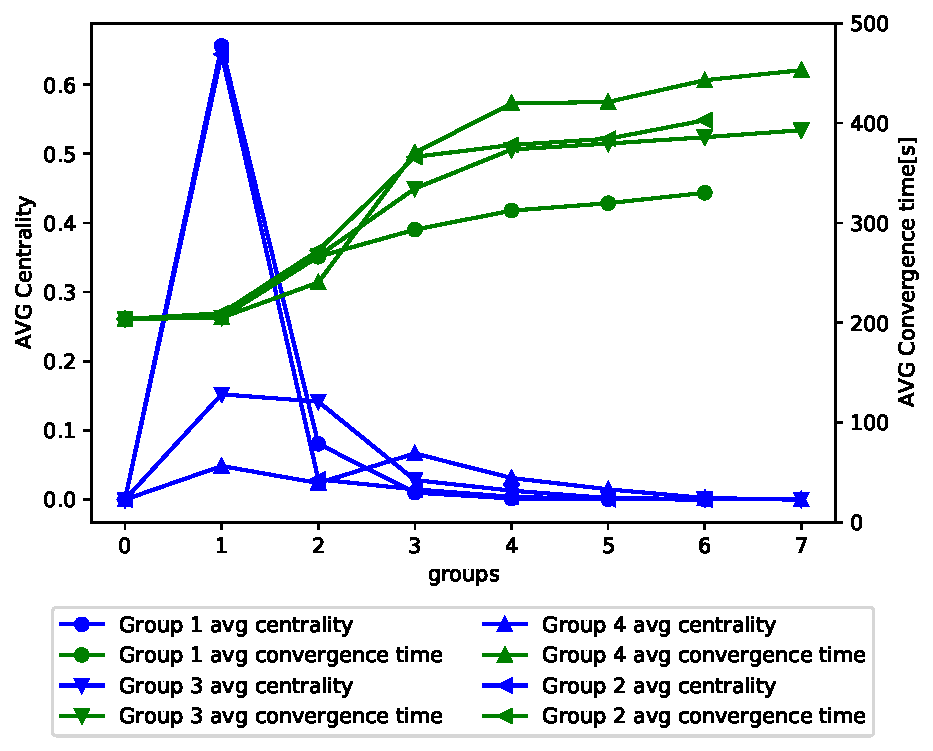
\includegraphics[width=\textwidth]{images/hierarchy/dpc_all_levels_comparison_centVStime.pdf}
		 \caption{\ac{MRAI} strategy \ac{DPC}, convergence time levels comparison}
         \label{fig:different_levels_comparison_dpc_time}
     \end{subfigure}
     \begin{subfigure}[b]{0.45\textwidth}
         \centering
         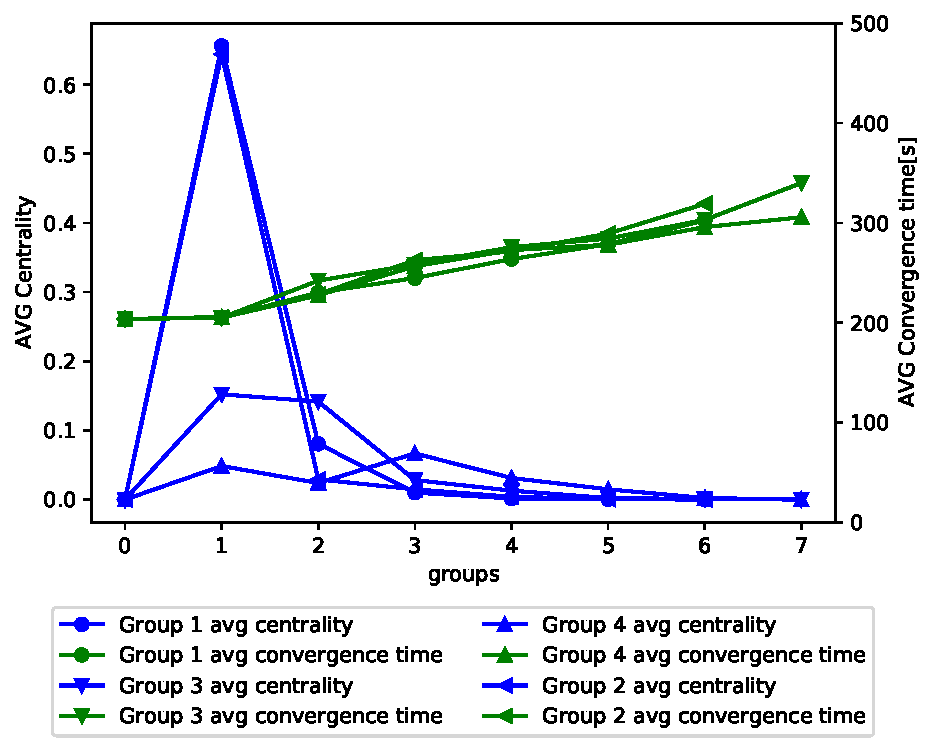
\includegraphics[width=\textwidth]{images/hierarchy/reverse_dpc_all_levels_comparison_centVStime.pdf}
		 \caption{\ac{MRAI} strategy reverse \ac{DPC}, convergence time levels comparison}
         \label{fig:different_levels_comparison_reverse_dpc_time}
     \end{subfigure}
     \hfill
	 \caption{Internet like topology of \num{1000} nodes grouped by the distance
	 from the signal source, different level comparison with \ac{MRAI} strategy
	 \ac{DPC} and reverse \ac{DPC}, \ac{MRAI} value equal to \SI{30}{\second}
	 \fxfatal{Maybe could be more interesting to see how \ac{DPC} vs \textit{Fixed}
	 goes}}
	 \label{fig:different_levels_comparison}
\end{figure}

In \Cref{fig:different_levels_comparison} is possible to see an analysis of the
average nodes performances grouped by the distance from the source of the signal.
Those performances are taken from the case where \ac{MRAI} is equal to
\SI{0}{\second}.
On the left side, is possible to see the performances of the nodes that uses the
\ac{DPC} \ac{MRAI} strategy, respectively
\Cref{fig:different_levels_comparison_dpc_msg,fig:different_levels_comparison_dpc_time}
while on the other side, \Cref{fig:different_levels_comparison_reverse_dpc_msg,fig:different_levels_comparison_reverse_dpc_time},
are showed the performances in case of a reverse \ac{DPC} strategy.

In all the figures in \Cref{fig:different_levels_comparison} the blue line
represents the average normalized centrality of the different nodes groups at different
levels. \fxfatal{Correct group in the plots with level}.
Is possible to see that in the case that the nodes are in the first or the
second level the nodes with the highest average centrality are the nearest ones.
While if the node is far away from the central clique the nodes with the
higher average centrality are in the second or third group.
The values for those groups are low because of the high number of nodes
in those groups, most of them having a small centrality value.
The centrality refers to the first y-axis on the left.

The two plots in \Cref{fig:different_levels_comparison_dpc_msg,fig:different_levels_comparison_reverse_dpc_msg},
respectively the \ac{DPC} case and the reverse \ac{DPC},
show the average number of messages required by each group of nodes to reach
the convergence state.
The main difference between them is in the number of messages experienced by
the nodes near the source.
In the \ac{DPC} case, the value remains stable around \num{10} messages, while,
with the reverse strategy, this number explodes up to \num{40} messages because
of the \textit{Path exploration} problem provoked by the central clique.

Is possible to notice that some of the lines end up at the $6^{th}$ group instead
of the $7^{th}$, that's because for the level \num{1} and \num{2} there are
no best paths to the destination that goes over the \num{6} hops.
The same behaviour is expected also for the convergence time performances.

Those ones are presented in \Cref{fig:different_levels_comparison_dpc_time,fig:different_levels_comparison_reverse_dpc_time}.
Is easily noticeable that with the \ac{DPC} strategy after the
more central groups there is a separation between the lines, but the trends
are the same.
The convergence time slowly increases in farthest nodes, thanks to the particular
\ac{MRAI} strategy that permits to wait for enough time to receive all the information
necessary.
This is also the reason for the small variance in terms of messages transmitted.
With the reverse \ac{DPC} strategy, on the other hand, is possible to have a
more stable trend in the convergence time that linearly grows.
This linear trend is caused by the fact that nodes could end up to send more
\ac{ADV} in order to correct a non best route.
This is one of the consequences of the \textit{Path Exploration} problem in
the central nodes.

Is then possible to conclude that the position of the node can highly impact
the \ac{MRAI} behaviour, signals from the periphery of the network can more
easily cause \ac{ADV} storms if \ac{MRAI} is not large enough to catch them.
Other than that, the position can influence the performances by itself, but
\ac{MRAI} can help to reduce the number of messages paying a higher convergence
time.

%\begin{itemize}
%    \item And how much is influencing the position?
%    \item Hierarchically?
%\end{itemize}
